\chapter{Bedarfsanalyse}
\label{cha:bedarfsanalyse}
In diesem Kapitel sollen die grundlegenden Prozesse des Shelf-Managements näher betrachtet werden. Dazu werden die Prozesse der Warenannahme, des Einräumens von Waren und der Kundenservice in einem Einzelhandel beispielhaft und ohne technische Unterstützung dargestellt, analysiert und anschließend Problemstellen aufgezeigt. Dabei wird insbesondere auf die Schwachstellen und Verbesserungspotenzial eingegangen.\\
Anschließend werden aus den Problemen und Schwachstellen Ziele definiert, die im weiteren Verlauf der Arbeit weiter analysiert und schließlich durch technologische Unterstützung erfüllt werden sollen.

\section{Warenannahme}
\label{cha:warenannahme}
Damit überhaupt Produkte in Regale eingeräumt werden können, muss die Ware zunächst in das Geschäft gelangen. Zunächst werden Waren durch geschultes Personal bestellt und anschließend nach einer gewissen Zeit von einem Transporter angeliefert. Die Waren werden üblicherweise auf Paletten verpackt, ein Lieferschein ist beigelegt. Sofern Ware bestellt und geliefert wurde, muss die Ware abgenommen werden. \glqq Abnehmen\grqq bedeutet in diesem Kontext, dass die Ware von der Filiale offiziell als geliefert gekennzeichnet wurde. Dazu gehört das Zählen der gelieferten Ware und der Abgleich mit den Positionen der Bestellung; hier wird überprüft, ob die Menge der bestellten Ware mit der gelieferten Menge übereinstimmt. Dazu wird eine sogenannte Setzliste verwendet, welche eine Kopie der Bestellung ist. Die Setzliste ist dabei nicht mit dem Lieferschein zu verwechseln.\\

Wurde die Palette abgearbeitet und die Setzliste abgehakt bzw. Differenzen zwischen Lieferung und Bestellung angegeben, wird diese zu einer Führungskraft des Geschäfts gebracht, damit diese die Setzliste offiziell unterzeichnet und dann in ein elektronisches System überträgt. Nach diesem Arbeitsschritt ist es möglich, in der Buchhaltung die entsprechenden Beträge zu verbuchen.\\

Solange die Ware nicht im Verkaufsraum benötigt wird, wird diese im Lager des Geschäfts aufbewahrt. Dieser Prozess ist in folgendem Aktivitätsdiagramm visualisiert und zeigt mögliche Fehlerquellen, Risiken und Problemstellen. Diese Erkenntnisse sind mithilfe von erfahrenen und sehr geschulten Führungskräften von einem führenden Einzelhändler in der eingangs erwähnten Studie erarbeitet worden.\\

\begin{figure}[H]
	\centering
	{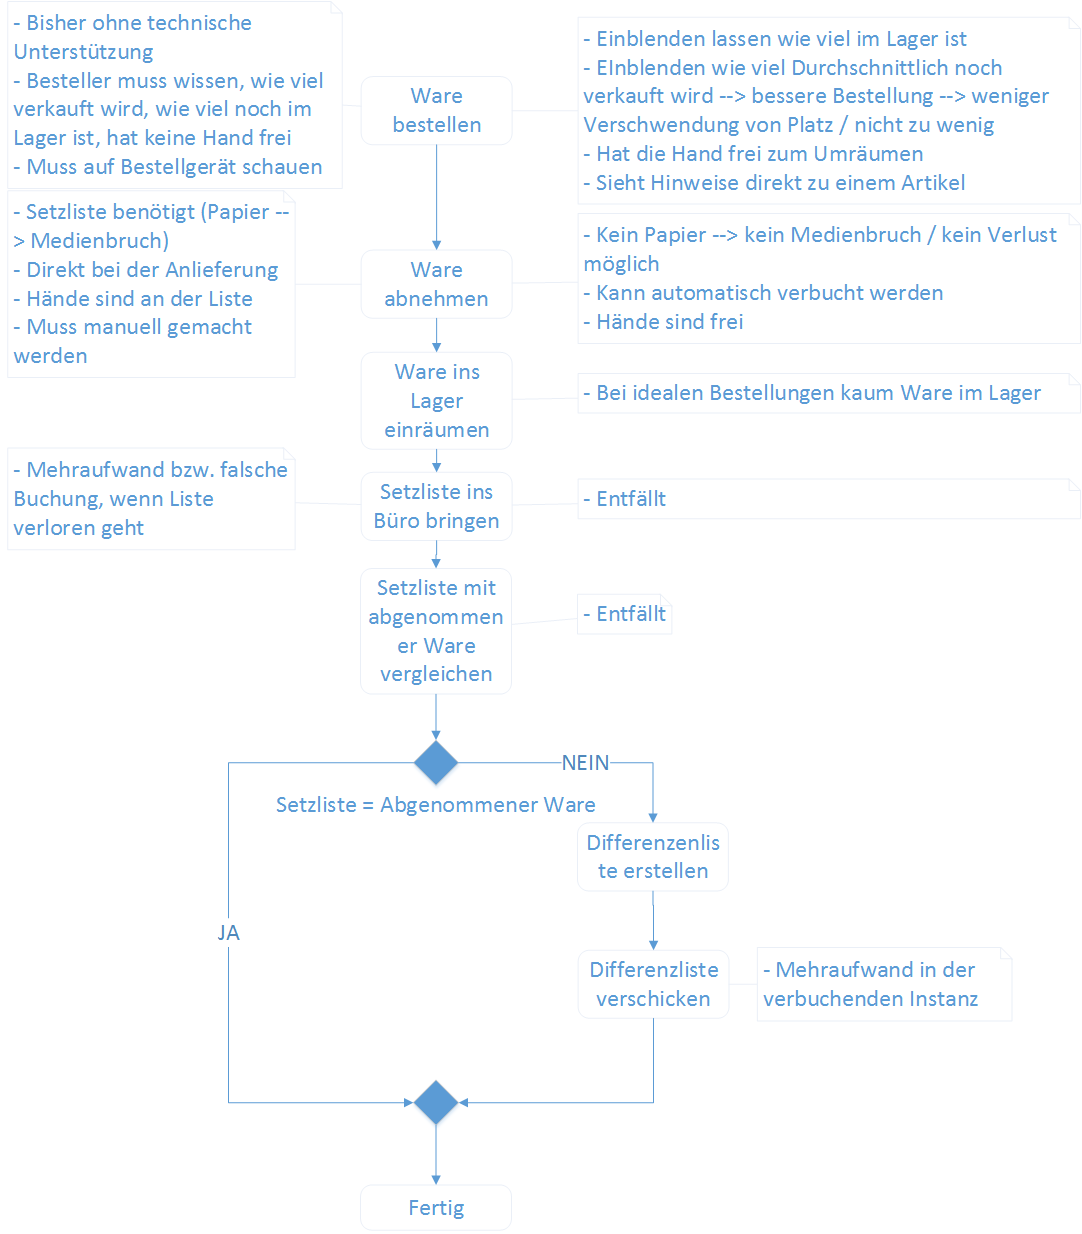
\includegraphics[scale=0.53]{Bilder/Abbildungen/Warenannahme_Vergleich.png}}
	\caption{Schematischer Ablauf der Warenannahme}
	\label{fig:warenannahme_vergleich}
\end{figure}

Wie in der Abbildung ersichtlich, fängt der Prozess bei der Bestellung von Waren an. Das verantwortliche Personal muss ohne technische Hilfsmittel selbst einschätzen können, welche Waren zum jeweiligen Zeitpunkt benötigt werden und in welchen Mengen diese Waren bestellt werden sollen. Dabei spielen verschiedene Aspekte eine große Rolle, etwa der Wochentag der Bestellung, das Wetter, die Jahreszeit, oder ob momentan Schulferien sind -- also alle Faktoren, die den Absatz einer Ware beeinflussen können. Beispielsweise ist während der Schulzeit die Käufergruppe der Schüler stärker vertreten als während der Ferienzeit, sodass bestimmte Waren stärker oder weniger nachgefragt werden.\\
Folglich ist es nur wenigen, erfahrenen Mitarbeitern möglich, eine sinnvolle Bestellung durchzuführen. Es ist allerdings wünschenswert, dass möglichst viele Mitarbeiter schnell bestellen können, sodass man unabhängiger von bestimmten Personen vor Ort wird, aber dennoch sorgfältige und sinnvolle Bestellungen tätigt.\\

Der Schritt \glqq Ware abnehmen\grqq erfordert die angesprochene Setzliste, welche auf Papier vorliegt. Dabei ist anzumerken, dass der Mitarbeiter durch das Abhaken der Setzliste keine Hand frei hat. Es wäre jedoch vorteilhaft, wenn der Mitarbeiter die Hände frei zum Arbeiten an der Palette hätte, um die Waren zu zählen. Außerdem können Fehler bei Bearbeitung der Setzliste geschehen, wie \zB ein Verzählen des Mitarbeiters. Zusätzlich sollte sofort bei Anlieferung die Ware überprüft werden, um die direkte Zuordnung zur Setzliste zu erhalten. So wird auch ein möglicher, unnötiger Verlust oder Beschädigung der Liste, und somit weitere Arbeit vermieden.\\
Angenommen, die Erfassung der Waren bei der Warenannahme würde durch eine entsprechende elektronische Lösung ersetzt, hätte der Mitarbeiter eine oder beide Hände immer frei zum Arbeiten. Da der Mitarbeiter, bei entsprechend automatisierter Warenerfassung, nicht mehr selbst zählen und vergleichen muss, ist die Fehlerwahrscheinlichkeit geringer als bei einer manuellen Erfassung und verspricht korrektere Buchungen sowie im Anschluss genauere Analysen. Außerdem ist es grundsätzlich schwieriger, eine elektronisch gespeicherte Liste zu verlieren.\\

Der nächste Arbeitsschritt, \glqq Ware in Lager einräumen\grqq , kostet in der Regel kaum Zeit, auch wenn er durch unerfahrenes Personal durchgeführt wird. Allerdings geht durch einen hohen Warenbestand im Lager viel Platz verloren, der im Idealfall besser genutzt werden könnte –- nämlich zum Verkauf von weiterer Ware, indem die Lagerfläche reduziert wird. Platz ist eine kostbare Ressource, wie man zum Beispiel an Grundstückspreisen feststellen kann. Außerdem besteht bei größerer Verkaufsfläche mehr Potential, den Umsatz zu erhöhen. Bei angemessenen Bestellungen und korrekten Lieferungen wird Ware sofort auf die Verkaufsfläche gestellt, sodass sie, im besten Fall, gar nicht erst im Lager aufbewahrt wird.\\

Wenn eine materielle Setzliste durch ein elektronisches Pendant abgelöst würde, entfielen Arbeitsprozesse wie \glqq Setzliste ins Büro bringen\grqq oder \glqq Setzliste mit abgenommener Ware vergleichen\grqq, sodass auch weiterer Mehraufwand durch verlorene oder falsche Lieferungen eingespart würde. Dabei ist anzumerken, dass der Aufwand bei falscher Lieferung zunächst nur in der Filiale entfällt. Die übergeordnete Instanz, die sich um die filialspezifischen Buchungen kümmert, muss dennoch die (Falsch-)Buchungen weiter arbeiten. Allerdings sind so die Daten schon von Beginn an digital erfasst und können ohne zusätzliches manuelles Eingreifen direkt weiter verarbeitet werden.

\section{Waren einräumen}
\label{waren_einräumen}
Während der Prozess der Warenannahme sich darauf beschränkt, die Ware vom Lieferanten entgegen zu nehmen und korrekt zu dokumentieren, behandelt das Shelf-Management das eigentliche Einräumen der Produkte in die Regale auf der Verkaufsfläche.\\

Ein Mitarbeiter muss die Ware aus dem Lager heraus an die richtige Stelle in den Regalen einräumen, und dies möglichst schnell, da sonst verderbliche Ware (wie \zB tiefgekühlte Lebensmittel) an Qualität verliert und insbesondere potenzieller Umsatz verloren geht, wenn Ware im Regal nicht vorrätig ist. Der Mitarbeiter nimmt die einzuräumende Ware im Normalfall auf einer Palette oder einem vergleichbar großen Container mit auf die Verkaufsfläche und stellt diese im Gang am Regal ab, um die Waren einzuräumen. Dabei steht er Kunden im Weg, die sich häufig über die Behinderung während des Einkaufs ärgern. Dies ist aus der Eingangs erwähnten Studie bei einem Einzelhändler hervorgegangen. Wenn der Kunde den Einräumprozess beobachtet und dabei der Mitarbeiter nicht genau weiß, wo die Ware eingeräumt werden muss, könnte der Kunde das Vertrauen an den Mitarbeiter und somit an den Händler. Dabei ist Kundenzufriedenheit ein wichtiger Aspekt, insbesondere dann, wenn der Kunde die Zufriedenheit mit dem Händler verliert. Daraus ergäben sich diese Folgen\footnote{\citep{controlling}}:
\begin{itemize}
	\item Unzufriedenheit führt zur Abwanderung bisheriger Kunden.
	\item Unzufriedene Kunden betreiben negative Mundpropaganda und berichten durchschnittlich zehn bis zwölf weiteren Personen von ihrer Unzufriedenheit.
	\item Die Gewinnung von Neukunden verursacht gegenüber der Bindung eines Altkunden das vier- bis sechsfache an Kosten.
\end{itemize}
Diese Folgen beziehen sich auf den Dienstleistungssektor, der nicht zu 100\% auf den Markt des Einzelhandels zutrifft. Allerdings sind die angesprochenen Punkte spätestens dann relevant, sobald der Kunde einen Mitarbeiter fragt, wo ein entsprechender Artikel auf der Verkaufsfläche zu finden ist \bzw ob dieser überhaupt vorhanden ist. Dann erfüllt der Mitarbeiter eine Dienstleistung an den Kunden, indem er ihm Auskunft gibt. Jedoch ist es sehr häufig der Fall, dass ein Mitarbeiter nicht weiß, ob oder wo ein Artikel vorhanden ist. Vor allem in Filialen mit großer Verkaufsfläche ist dies der Fall.\\

Es besteht also sowohl im Sinne der Kundenzufriedenheit als auch zur Steigerung der Effizienz Optimierungspotenzial im Einräumprozess, welches durch elektronische Unterstützung genutzt werden könnte. Vor allem bei einer großer Verkaufsfläche, vielen Regalen und vielen Artikeln ist es für gerade für unerfahrene Mitarbeiter schwer zu erkennen, wo genau der Artikel eingeräumt werden muss. Bei wechselnden Sortierungen ist es selbst für erfahrene Mitarbeiter schwierig, den aktuellen Standort eines Artikels zu wissen. Gerade beim Shelf-Management wäre es zudem wichtig, dass der Mitarbeiter beide Hände frei hat zum Arbeiten.

\section{Kundenservice}
Aus der selbst durchgeführten Studie ging auch hervor, dass Mitarbeiter (insbesondere in großen Filialen) dem Kunden auf Anfrage nicht beantworten können, ob ein bestimmtes Produkt noch vorrätig ist oder wo es auf der Verkaufsfläche zu finden sei. Generell lässt sich genau durch dieses Wissen die zuvor angesprochene Kundenzufriedenheit erhöhen. Da diese Schwachstelle den zuvor angesprochenen sehr stark ähnelt, soll diese auch im weiteren Verlauf der Arbeit thematisiert werden. 

\section{Zieldefinition}
\label{sec:zieldefinition}
Aus den genannten Arbeitsprozessen ergeben sich also mehrere potenzielle Problembereiche des konventionellen Shelf-Managements:

\begin{itemize}
	\item Der Mitarbeiter muss erkennen, wann er welche Ware einräumen muss.
	\item Der Mitarbeiter muss wissen, wo er die Ware einzuräumen hat.
	\item Der Mitarbeiter muss wissen, wie viel von der Ware generell noch vorhanden ist.
	\item Der Kundenservice kann unter mangelnden Kenntnissen der Mitarbeiter über aktuelle Zustände in der Filiale leiden.
\end{itemize}

Diese Schwachstellen zeigen auf, dass es in allen Arbeitsschritten von der Warenannahme bis zum Verkauf Optimierungspotenzial gibt. Es gibt also einen Bedarf zur Verbesserung der Warenannahme und des Shelf-Managements. In den genaueren Erläuterungen wurde auch herausgestellt, dass durch Einsatz entsprechender technologischer Lösungen viele Probleme vermieden werden können und die Effizienz gesteigert werden kann.\\
Das Hauptziel dieser Arbeit soll daher sein, eine technische Lösung zu entwickeln, die diese Probleme angeht und die Arbeitsprozesse verbessert. Daraus lassen sich konkretere Unterziele ableiten:

\begin{itemize}
	\item Die Arbeitsgeschwindigkeit eines Mitarbeiters soll beim Einräumen von Ware erhöht werden, vor allem bei ungeschultem Personal.
	\begin{itemize}
		\item Der Mitarbeiter soll beim Einräumen der Ware technisch unterstützt werden.
	\end{itemize}
	\item Der Mitarbeiter soll bei der Warenannahme entlastet und die Fehleranfälligkeit des Prozesses verringert werden.
	\begin{itemize}
		\item Bestellungen sollen elektronisch verwaltet werden können.
		\item Gelieferte Ware soll durch eine technische Lösung optimaler erfasst werden können.
	\end{itemize}
	\item Die Kundenzufriedenheit in der Filiale soll erhöht werden.
	\begin{itemize}
		\item Der Mitarbeiter soll in der Lage sein, dem Kunden den Platz eines bestimmten Artikels nennen zu können.
		\item Der Mitarbeiter soll in der Lage sein, dem Kunden den Lagerbestand eines Artikels nennen zu können. 
	\end{itemize}
\end{itemize}
